% Opening packages ---------------------------------

\documentclass[12pt, a4paper]{article}
\parindent 0px
\parskip=10pt
\usepackage[utf8]{vietnam}
\usepackage[left=1.20cm, right=1.20cm, top=1.50cm, bottom=1.50cm]{geometry}
\usepackage{amsmath,amssymb,amsfonts}
\usepackage{gensymb}
\usepackage{enumitem}
\usepackage{multicol}
\usepackage{graphicx}
\usepackage{array}
\usepackage{float}
\usepackage[onehalfspacing]{setspace}
\usepackage{mathpazo}
\usepackage{wrapfig}

% Title --------------------------------------------


\title{\vspace{-1.5cm}{\huge\textbf{Chuyên đề: Khảo sát hàm số}}\\[3mm]
		{\LARGE Khối lớp: 12}\\[2mm]
		{\LARGE Thời gian: 45 phút}\\[1mm]
{\normalsize Họ và tên~\rule{3cm}{1pt} \hfill Điểm: ~\rule{1cm}{1pt}}\\[4mm]
\hrule
}
\author{}
\date{}

% Bắt đầu đề---------------------------------------

\begin{document}
	\maketitle
	\vspace{-2.15cm}

\end{document}

% ------------------------------------------------

% 4 cột

	\begin{multicols}{4}
		\begin{enumerate}
			\item[\textbf{A.}]
			\item[\textbf{B.}] 
			\item[\textbf{C.}] 
			\item[\textbf{D.}] 
		\end{enumerate}
	\end{multicols}

% 2 cột

	\begin{multicols}{2}
		\begin{enumerate}
			\item[\textbf{A.}]
			\item[\textbf{C.}] 
			\item[\textbf{B.}] 
			\item[\textbf{D.}] 
		\end{enumerate}
	\end{multicols}
	
% 1 cột

\vspace{-0.5cm}
	\begin{enumerate}
		\item[\textbf{A.}]
		\item[\textbf{B.}] 
		\item[\textbf{C.}] 
		\item[\textbf{D.}] 
	\end{enumerate}
	
% Trắc nghiệm đúng sai 

\vspace{-0.5cm}
	\begin{enumerate}
		\item[\textbf{a)}]
		\item[\textbf{b)}] 
		\item[\textbf{c)}] 
		\item[\textbf{d)}] 
	\end{enumerate}

% Làm bảng ---------------------------------------

\begin{table}[H]
	\centering
	\def\arraystretch{2.5}
		\begin{tabular}{|p{15cm}||c|c|} \hline
			\multicolumn{1}{|c||}{\textbf{Mệnh đề}} &\textbf{Đúng} & \textbf{ Sai \, }\\ \hline
			\textbf{a.}  & & \\ \hline
			\textbf{b.}  & & \\ \hline
			\textbf{c.}  & & \\ \hline
			\textbf{d.}  & & \\ \hline
		\end{tabular}
\end{table}

% Cách vẽ bảng biến thiên (\usepackage{tkz-tab}) ------------------------

\begin{center}
		
\begin{tikzpicture}
			\tkzTabInit[nocadre = false , lgt = 2 , espcl = 2]
				{ $ x $ / 1 , $ f'(x) $ / 1 , $ f(x) $ / 2 }
				{ $ - \infty $ , $ -2 $ , $ -1 $ , $ 0 $ , $ + \infty $ } 
			\tkzTabLine
				{ , + , $ 0 $ , - , d , + , $ 0 $ , - , }
			\tkzTabVar
				{ +/ $ 2 $ , -/ $ -4 $ , +/ $ 1 $ , -/ $ 0 $ , +/ $ 3 $ }
		\end{tikzpicture}
\end{center}	

% Trả lời ngắn -----------------------------------

\textbf{Câu : } 

	\textit{\textbf{Đáp số: }}
	\framebox[20mm]{\rule{0pt}{4mm}}

% Tự luận (\usepackage{linegoal}) ---------------------

\makeatletter

\newcommand*\dotcolumnfill{%
    \par\noindent\mbox{}\@tempdima=\dimexpr\linewidth-\linegoal
    \null
    \vskip -\ht\strutbox
    \xleaders \hb@xt@ \hsize {%     
        \hspace{\@tempdima}\strut \leavevmode \cleaders \hb@xt@ .44em{\hss.\hss}\hfill
    }\vfill
    \vskip \ht\strutbox
    \break
}

\makeatother

% Begin thêm vào 

\makeatother

% GTLN - GTNN ------------------------------------

$\displaystyle\max_{\substack{[1;3]}} f(x)$

% Thêm footer vào beginning cho đề cương ôn tập -------

\fancyfoot[R]{\thepage}

% Vẽ đồ thị hàm số \usepackage{tkz-tab}--------------------------------

\begin{center}
		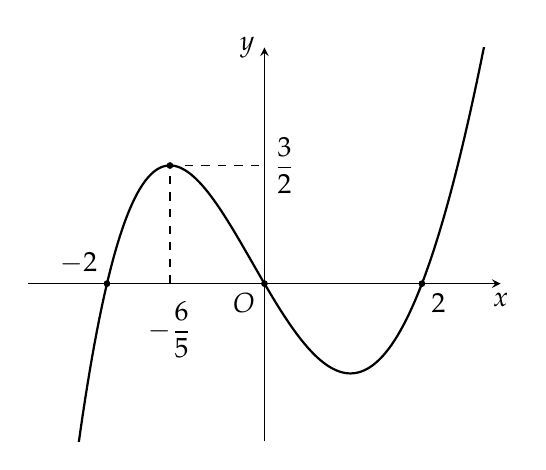
\begin{tikzpicture}[ >=stealth ]	
		
% Trục Oxy

    \draw[->] (-3 , 0) -- (3 , 0);   % X-axis
    \draw[->] (0 , -2) -- (0 , 3);   % Y-axis
    \draw (0 , 0) node[below left] { $O$ };  
    \draw (3 , 0) node[below] { $x$ };
    \draw (0 , 3) node[left] { $y$ };

% Đánh số

    \draw (-1.2 , -0.1) node[below] { $ -\dfrac{6}{5} $ };
    \draw (-2 , 0) node[above left] { $ -2 $ };
    \draw (2 , 0) node[below right] { $ 2 $ };
    \draw (0 , 1.5) node[right] { $ \dfrac{3}{2} $ }; 
    
% Dấu gạch nối

	\draw[dashed] (-1.2 , 0) -- (-1.2 , 1.5) -- (0 , 1.5);
    
% Dấu chấm

    \filldraw (-1.2, 1.5) circle (1pt);   
    \filldraw (-2, 0) circle (1pt);       
    \filldraw (2, 0) circle (1pt);        
    \filldraw (0, 0) circle (1pt);       
    
% Giới hạn y

    \clip (-3,-2) rectangle (3,3);

 % Hàm
 
    \draw[thick, samples=200, domain=-3:3] 
        plot(\x, {-0.0509 * \x * (\x - 2) * (\x + 2) * (\x - 8.4) });
        
		\end{tikzpicture}
	\end{center}
	
% Hàm số có n đoạn phân biệt --------------------

	$
	f(x) =
	\begin{cases}
	    \dfrac{x + \sqrt{x} - 2}{\sqrt{x} - 1} & \text{khi } x \geq 1 \\
	    -x^2 - 2x + 6 & \text{khi } x < 1
	\end{cases}
	$
	
% Nguyên hàm tích phân -------------------------

$ \displaystyle \int\limits_{-1}^{1} 0 \; \mathrm{d}x = C $

% Hình ảnh kế đề-------------------------------

\begin{minipage}{0.7\textwidth}
    \noindent
    \textbf{Câu 2:} Cho hàm số $y = \dfrac{ax^2 + bx + c}{mx + n}$ \, $(\text{với } a \neq 0; \, m \neq 0)$ có đồ thị như hình vẽ bên dưới đây. Phương trình đường tiệm cận xiên của đồ thị hàm số đã cho là:
    
% Hai cột đáp án
    \begin{multicols}{2}
        \begin{enumerate}
            \item[\textbf{A.}] $y = x - 2$
            \item[\textbf{B.}] $y = 2x + 2$
            \item[\textbf{C.}] $y = 2x - 2$
            \item[\textbf{D.}] $y = x + 2$
        \end{enumerate}
    \end{multicols}
\end{minipage}%
\hfill
\begin{minipage}{0.3\textwidth}
    \centering
    \includegraphics[scale=0.5]{1} % Thay "1" bằng tên file hình ảnh
\end{minipage}

% Vẽ bảng -----------------------------------------

	\begin{table}[h!]
		\centering
		\renewcommand{\arraystretch}{1.5}
			\begin{tabular}{|c||c|c|c|c|}
				\hline
				Cân nặng (kg) & $ [1,0; 1,1) $ & $ [1,1; 1,2) $ & $ [1,2; 1,3 ) $ & $ [1,3; 1,4) $ \\ \hline
				Số con giống A  & 8   & 28  & 32  & 17      \\ \hline 
				Số con giống B  & 13  & 14  & 24  & 14      \\ \hline
			\end{tabular}
	\end{table}